%%%%%%%%%%%%%%%%%%%%%%%%%%%%%%%%%%%%%%%%%%%%%%%%%%%%%%%%%%%%%%%%%%%%%%%%%%%%%%%%
%%                          uAlberta Thesis Template                          %%
%%                                     by                                     %%
%%                               Daniel Aldrich                               %%
%%                               Version: 1.0.0                               %%
%%%%%%%%%%%%%%%%%%%%%%%%%%%%%%%%%%%%%%%%%%%%%%%%%%%%%%%%%%%%%%%%%%%%%%%%%%%%%%%%
%                                                                              %
%       Copyright (c) 2019 Daniel Aldrich                                      %
%                                                                              %
%       Permission is hereby granted, free of charge, to any person            %
%       obtaining a copy of this software and associated documentation         %
%       files (the "Software"), to deal in the Software without                %
%       restriction, including without limitation the rights to use,           %
%       copy, modify, merge, publish, distribute, sublicense, and/or           %
%       sell copies of the Software, and to permit persons to whom the         %
%       Software is furnished to do so, subject to the following               %
%       conditions:                                                            %
%                                                                              %
%       The above copyright notice and this permission notice shall be         %
%       included in all copies or substantial portions of the Software.        %
%                                                                              % 
%       THE SOFTWARE IS PROVIDED "AS IS", WITHOUT WARRANTY OF ANY KIND,        % 
%       EXPRESS OR IMPLIED, INCLUDING BUT NOT LIMITED TO THE WARRANTIES        %
%       OF MERCHANTABILITY, FITNESS FOR A PARTICULAR PURPOSE AND               % 
%       NONINFRINGEMENT. IN NO EVENT SHALL THE AUTHORS OR COPYRIGHT            %
%       HOLDERS BE LIABLE FOR ANY CLAIM, DAMAGES OR OTHER LIABILITY,           %
%       WHETHER IN AN ACTION OF CONTRACT, TORT OR OTHERWISE, ARISING           %
%       FROM, OUT OF OR IN CONNECTION WITH THE SOFTWARE OR THE USE OR          %
%       OTHER DEALINGS IN THE SOFTWARE.                                        %
%                                                                              %
%%%%%%%%%%%%%%%%%%%%%%%%%%%%%%%%%%%%%%%%%%%%%%%%%%%%%%%%%%%%%%%%%%%%%%%%%%%%%%%%
%                                                                              %
%                                   NOTICE                                     %
% This template and class assume a basic understanding of how LaTeX works.     %
%                                                                              %
%%%%%%%%%%%%%%%%%%%%%%%%%%%%%%%%%%%%%%%%%%%%%%%%%%%%%%%%%%%%%%%%%%%%%%%%%%%%%%%%
%                                                                              %
% To use this template start by entering in your information in the fields     %
%     below, and in the file `ualberta.xmpdata'. Next remember to delete the   %
%     auto genterated text `\lipsum[##]'.                                      %
%                                                                              %
% Most LaTeX packages required have already been included in this document     %
%     document class.                                                          %
%                                                                              %
% For referencing, use the command \Cref{<label>} for smart referencing that   %
%     includes the type of reference, i.e., for a figure it will produce the   %
%     the text `Figure #.#'.                                                   %
%                                                                              %
% Compact citations can be made by using a single \cite command, e.g.:         %
%     `\cite{ref1, ref2, ref3,...}.                                            %
%                                                                              %
%%%%%%%%%%%%%%%%%%%%%%%%%%%%%%%%%%%%%%%%%%%%%%%%%%%%%%%%%%%%%%%%%%%%%%%%%%%%%%%%

% INCLUDES PACKAGES:
% array, nomencl, etoolbox, lipsum, xmpincl, xcolor, graphicx, tabularx, 
%  makecell, subcaption, rotating, booktabs, multicol, multirow, amsmath, 
%   amsfonts, amssymb, pdflscape, textcomp, longtable, listings, pdfpages
%    xparse, ifthen, hyphenat, hyperref, cleveref, inputenc
% 
% For a full description of each of the included packages please read the 
%  packages file.

%LIST OF DEFINED SYMBOLS
        %\regTM                %Registered Trademark\regTM
        %\nonTM                %Unregistered Trademark
        %\cRight{}             %Copyright
        %\cLeft{}              %Copyleft
        %\degrees{}            %Degrees
        %\hyph{}               %Hyphen
        %\latin{<text here>}   %Latin
        %\etal{}               %et al.
        %\etc{}                %etc
        %\eg{}                 %e.g.
        %\ie{}                 %i.e.
        %\Kevlar{}             %Kevlar
        %\Matlab{}             %Matlab

%LIST OF AVAILABLE THEOREM ENVIRONMENTS
        % theorem, algorithm, axium, case, claim, conclusion, condition, 
        % conjecture, corollary, criterion, definition, example, exercise, 
        % lemma, notation, problem, proposition, remark, solution, summary
        %
        % To use:
        % \begin{<theorem name>}
        %   <YOUR TEXT HERE>
        % \end{<theorem name>}
        
%LIST OF USEFUL COMMANDS:
        %\comment{}            %Nothing inside the braces will be printed
        %\nonumeq{}            %Un-numbered, centered equation.
        %\numeq{}{label}       %Numbered, centered equation.
        %\brackS{}             %Surrounds the input with []
        %\brackR{}             %Surrounds the input with ()
        %\brackC{}             %Surrounds the input with {}

% INCLUDING CODE
	   % To include code or code snippets in your thesis, the package listings is used.
	   % A number of predefined code highlighting schemes are included in the file
	   %   listingCodeFormatting.tex including:
	   %   Matlab, C/C++, VB/VBA, and XML 
	   %
	   % Examples of how to include code are shown in Appendix C

\immediate\write18{makeindex \jobname.nlo -s nomencl.ist -o \jobname.nls}
% Write command to allow the nomenclature to be generated properly.


\documentclass[pdfa,chapterbib]{ualberta}
% OPTIONS FOR ualberta.cls:
% chapterbib - \printreferences now prints references at the end of a chapter
% 
% pdfa - to convert the pdfa to PDF/A format
% 
% oneside - Standard for submitting to FGSR.
% 
% twoside - If you want to print your thesis double sided.

%%%%%%%%%%%%%%%%%%%%%%%%%%%%%%%%%%%%%%%%%%%%%%%%%%%%%%%%%%%%%%%%%%%%%%%%%%%%%%%%
%                  TITLE PAGE AND FRONTMATTER INFORMATION                      %
%%%%%%%%%%%%%%%%%%%%%%%%%%%%%%%%%%%%%%%%%%%%%%%%%%%%%%%%%%%%%%%%%%%%%%%%%%%%%%%%
% TITLE PAGE INFO
 \title{Thesis Title}              % Title of your Thesis
 \author{First Middle Last}        % Your Full Name
 \degree{\MSc}                     % \MSc or \PhD
 \specialization{}                 % Leave blank if none
 \department{Example Department}   % Department you are completing your degree
 \convocationdate{Term YYYY}       % Term (Fall, Winter, Spring)

% Don't forget to edit ualberta.xmpdata with the same metadata for the PDF/A

% FRONTMATTER INFO
 \abstracttext{\lipsum[4-7] }
 \preface{This thesis is an original work by `Your name here'. No part of this thesis has been previously published.}
 \thesisquote{``\lipsum*[14]{}''\\-Author of the Quote}
 \dedication{To...}
 \acknowledgementtext{\lipsum[2-3]}


%%%%%%%%%%%%%%%%%%%%%%%%%%%%%%%%%%%%%%%%%%%%%%%%%%%%%%%%%%%%%%%%%%%%%%%%%%%%%%%%
%                  NOMENCLATURE, GLOSSARY, ACRONYMS, ETC                       %
%%%%%%%%%%%%%%%%%%%%%%%%%%%%%%%%%%%%%%%%%%%%%%%%%%%%%%%%%%%%%%%%%%%%%%%%%%%%%%%%

% NOMENCLATURE
 % [A] : Constants
 % [B] : Latin
 % [C] : Greek
 % Use \nomunit{Value, Units} to add the value and units for a defined constant

 \nomenclature[A]{$c$}{Speed of light in a vacuum inertial system.\nomunit{$299,792,458\, m/s$}}
 \nomenclature[B]{$E$}{Elastic Constant (Young's Modulus)}
 \nomenclature[C]{$\alpha$}{Strain}

% ACRONYMS
 \addacronym{t}{stands for test}

% GLOSSARY
 \addterm{test}{this is a test}

% BIBLIOGRAPHY LOCATION
 % .  - This folder
 % .. - Up one Folder
 \addbibresource{./References/References.bib}


%%%%%%%%%%%%%%%%%%%%%%%%%%%%%%%%%%%%%%%%%%%%%%%%%%%%%%%%%%%%%%%%%%%%%%%%%%%%%%%%
%                              BEGIN DOCUMENT                                  %
%%%%%%%%%%%%%%%%%%%%%%%%%%%%%%%%%%%%%%%%%%%%%%%%%%%%%%%%%%%%%%%%%%%%%%%%%%%%%%%%
\begin{document}

 \maketitle                    % Creates the title page
 \makeabstract                 % Creates the abstract
 \makepreface                  % Uncomment line to add Preface Page
 %\makequote                   % Uncomment line to add Quote Page
 %\makededication              % Uncomment line to add Dedication Page
 \acknowledgements             % Uncomment line to add Acknowledgements
 \tableofcontents              % Create the Table of Contents
 \listoftables                 % Uncomment line if you have tables
 \listoffigures                % Uncomment line if you have figures
 \listofplates                 % Uncomment line if you have plates (photographs)
 %\listofsymbols               % Uncomment if you have a List of Symbols (Nomenclature)
 %\abbreviations               % Uncomment if you have a List of Acronyms
 \glsaddall                    % Required for List of Acronyms and Glossary (DO NOT COMMENT)
 %\generateglossary            % Uncomment if you have Glossary
 \bodyoftext                   % Switches the style of the document to that required for the body

% SET DOCUMENT SPACING
 %\onehalfspacing        
 \truedoublespacing
 %\triplespacing

%%%%%%%%%%%%%%%%%%%%%%%%%%%%%%%%%%%%%%%%%%%%%%%%%%%%%%%%%%%%%%%%%%%%%%%%%%%%%%%%
%                           ADD YOUR CONTENT HERE                              %
%%%%%%%%%%%%%%%%%%%%%%%%%%%%%%%%%%%%%%%%%%%%%%%%%%%%%%%%%%%%%%%%%%%%%%%%%%%%%%%%
\chapter{Introduction}\label{ch:Introduction}
  \lipsum[6-8]
  \section{Motivation}\label{sec:Motivation}
    \lipsum[1-3]
  \section{Thesis Objectives}\label{sec:thesisObjective}
    \lipsum[14-16]
  \section{Thesis Outline}\label{sec:thesisOutline}
    \lipsum[17]
                
\chapter{Background}\label{ch:Background}
  \section{General Information}\label{sec:}
    \lipsum[23-25]
  \section{Specific Information}\label{sec:}
    \lipsum[35-37]
  \section{Gap in Research}\label{sec:}
    \lipsum[42-43]
  \section{Conclusions}\label{sec:}
    \lipsum[12-13]

\chapter{Paper 1}\label{ch:Paper1}
  \section{Introduction}\label{sec:}
    \lipsum[34-36]
  \section{Methods and Procedure}\label{sec:}
    \begin{case}
      \lipsum[10]
    \end{case}
    \begin{case}
      \lipsum[15]
    \end{case}
    \lipsum[46-48]
  \section{Results and Discussion}\label{sec:}
    \lipsum[55-57]
  \section{Conclusions}\label{sec:}
    \lipsum[12-13]
                
\chapter{Paper 2}\label{ch:Paper2}
  \section{Introduction}\label{sec:}
    \lipsum[34-36]
  \section{Methods and Procedure}\label{sec:}
    \lipsum[46-48]
  \section{Results and Discussion}\label{sec:}
    \lipsum[55-57]
  \section{Conclusions}\label{sec:}
    \lipsum[12-13]
                
\chapter{Conclusions, Recommendations, \& Future Work}\label{ch:Conclusions}
  \section{Conclusions}\label{sec:}
    \lipsum[34-36]
  \section{Future Work}\label{sec:}
    \lipsum[38]\cite{TEST}
        % \printreferences Prints a reference section at the end of the current chapter
        %
        % If the `chapterbib' option is not declaired, \printreferences does nothing
        %    This allows you to turn end of chapter references on and off easily.
        %
        % Note: End of chapter references share references with the Bibliography that
        %    is required at the end of your thesis, so the numbering of the end of 
        %    chapter references may not start at one and may not increment by one.
        \printreferences 
\chapter{Example Chapter}\label{ch:Example}
  This chapter aims to provide examples how how to structure and create specific components in your thesis document. 
  The very first one is showing a citation, like the one at the end of this sentence \cite{TEST}. 
  The second shows how to create more than one citation and how they are grouped \cite{testone,cite2,cite3,cite4,cite5}.
  This sentence shows how a gap in the citations is handled \cite{testone,cite2,cite3,cite5}. 
  \section{Tables}
	
  % X - Justified (Equal Spacing)
  % L - Left Aligned (Equal Spacing)
  % C - Center Aligned (Equal Spacing)
  % R - Right Aligned (Equal Spacing)
  % l - Left Aligned (Fit to Contents)
  % c - Center Aligned (Fit to Contents)
  % r - Right Aligned (Fit to Contents)
  
  \begin{table}[!htb]
    \caption{This is a basic table}
    \centering
    \begin{tabularx}{0.75\textwidth}{LCR} 
      % Equally spaced cells that are left, center, and right aligned. 
      % The entire table will be 75% the width of the text.
      \hline
      \textbf{Left Aligned Title} & \textbf{Centered Title} & \textbf{Right Aligned Title} \\\hline
      This is left aligned & This is centered & This is right aligned \\
      This is left aligned & This is centered & This is right aligned \\
      This is left aligned & This is centered & This is right aligned \\
      This is left aligned & This is centered & This is right aligned \\\hline
    \end{tabularx}
    \label{tab:basicTable}
  \end{table}
  
  \begin{table}[!htb]
    \caption{This is a complex table.}
    \centering
    \begin{tabularx}{\textwidth}{lCR}
      % Left most cell is fitted to the content.
      % The center and right columns are equally spaced cells that are center, and right aligned. 
      % The entire table will be 75% the width of the text.
      \hline
      \multirow{2}{*}{\textbf{This is two row\quad}} & \multicolumn{2}{c}{\textbf{This is two columns}}\\\cline{2-3} % \cline draws a partial line across cells #-#
       & \textbf{Centered Title} & \textbf{Right Aligned Title} \\\hline
      \multirow{2}{*}{This is two row} & This is centered & This is right aligned \\
       & This is centered & This is right aligned \\\cline{1-1}
      \multirow{2}{*}{This is two row} & This is centered & This is right aligned \\
       & This is centered & This is right aligned \\\hline
    \end{tabularx}
    \label{tab:complexTable}
  \end{table}
  
  
  \section{Figures}
  This section will provide examples of how to create figures, and different types of multi/sub-figures. 
  Additionally, if you have many figures in a section and they are bleeding too much into the following sections a \texttt{\textbackslash{}clearpage} command can be issued before the next section. 
  However, note that this will force the next section to begin on a new page. 
  Note that the first ``figure'' is actually a plate; a plate is the proper title associated with a \textit{photograph}, using the environment `plate' instead of `figure' and command \texttt{\textbackslash{listofplates}} will generate everything for you.
  \begin{plate}[!htb]
    \centering
    \includegraphics[width=0.7\textwidth]{example-image}
    \caption{This is an example of a single image plate.}
    \label{fig:singleImage}
  \end{plate}
  
  \begin{figure}[!htb]
    \centering
    \begin{subfigure}{0.45\textwidth}
      \includegraphics[width=\textwidth]{example-image}
      \caption{} % Leave blank for just letter
      \label{fig:doubleImage:a}
    \end{subfigure}
    ~
    \begin{subfigure}{0.45\textwidth}
      \includegraphics[width=\textwidth]{example-image}
      \caption{} % Leave blank for just letter
      \label{fig:doubleImage:b}
    \end{subfigure}
    \caption{This is an example of a double image figure.}
    \label{fig:doubleImage}
  \end{figure}
  
  \begin{figure}[!htb]
    \centering
    \hspace*{\fill}% Adds space to left of top image (prevents two images from going to top)
    \begin{subfigure}{0.45\textwidth}
      \includegraphics[width=\textwidth]{example-image}
      \caption{} % Leave blank for just letter
      \label{fig:tripleImage:a}
    \end{subfigure}
    \hspace*{\fill} % Adds space to right of top image (prevents two images from going to top)
    \par\vspace{1em}% Adds space between upper and lower images
    \begin{subfigure}{0.45\textwidth}
      \includegraphics[width=\textwidth]{example-image}
      \caption{} % Leave blank for just letter
      \label{fig:tripleImage:b}
    \end{subfigure}
    ~ % Adds space between the two lower figures
    \begin{subfigure}{0.45\textwidth}
      \includegraphics[width=\textwidth]{example-image}
      \caption{} % Leave blank for just letter
      \label{fig:tripleImage:c}
    \end{subfigure}
    \caption{This is an example of a triple image figure.}
    \label{fig:tripleImage}
  \end{figure}
  
  \begin{figure}[!htb]
    \centering
    \hspace*{\fill}% Adds space to left of top image (prevents two images from going to top)
    \begin{subfigure}{0.90\textwidth+1em} % 0.9 = 0.45 + 0.45, and 1em is the width of ~
      \includegraphics[width=\textwidth]{example-image}
      \caption{} % Leave blank for just letter
      \label{fig:tripleImage:a}
    \end{subfigure}
    \hspace*{\fill} % Adds space to right of top image (prevents two images from going to top)
    \par\vspace{1em}% Adds space between upper and lower images
    \begin{subfigure}{0.45\textwidth}
      \includegraphics[width=\textwidth]{example-image}
      \caption{} % Leave blank for just letter
      \label{fig:tripleImage:b}
    \end{subfigure}
    ~ % Adds space between the two lower figures
    \begin{subfigure}{0.45\textwidth}
      \includegraphics[width=\textwidth]{example-image}
      \caption{} % Leave blank for just letter
      \label{fig:tripleImage:c}
    \end{subfigure}
    \caption{This is a second example of a triple image figure.}
    \label{fig:tripleImage}
  \end{figure}
  
  \begin{figure}[!htb]
    \centering
    \begin{subfigure}{0.45\textwidth}
      \includegraphics[width=\textwidth]{example-image}
      \caption{} % Leave blank for just letter
      \label{fig:quadImage:a}
    \end{subfigure}
    ~ % Adds space between the two top figures
    \begin{subfigure}{0.45\textwidth}
      \includegraphics[width=\textwidth]{example-image}
      \caption{} % Leave blank for just letter
      \label{fig:quadImage:b}
    \end{subfigure}
    \par\vspace{1em} % Adds space between upper and lower images
    \begin{subfigure}{0.45\textwidth}
      \includegraphics[width=\textwidth]{example-image}
      \caption{} % Leave blank for just letter
      \label{fig:quadImage:c}
    \end{subfigure}
    ~ % Adds space between the two lower figures
    \begin{subfigure}{0.45\textwidth}
      \includegraphics[width=\textwidth]{example-image}
      \caption{} % Leave blank for just letter
      \label{fig:quadImage:d}
    \end{subfigure}
    \caption{This is an example of a quad image figure.}
    \label{fig:quadImage}
  \end{figure}
  
  \clearpage % forces the remaining images (floats to be placed)
  \section{Graphs \& Plots}
  In the following section there will be a few examples of how to generate plots.
  For more information on how to create plots, \href{https://mirror.its.dal.ca/ctan/graphics/pgf/contrib/pgfplots/doc/pgfplots.pdf}{\textcolor{blue}{\underline{here}}} is the manual for pgfplots.
  \begin{figure}[htb!]
    \centering
    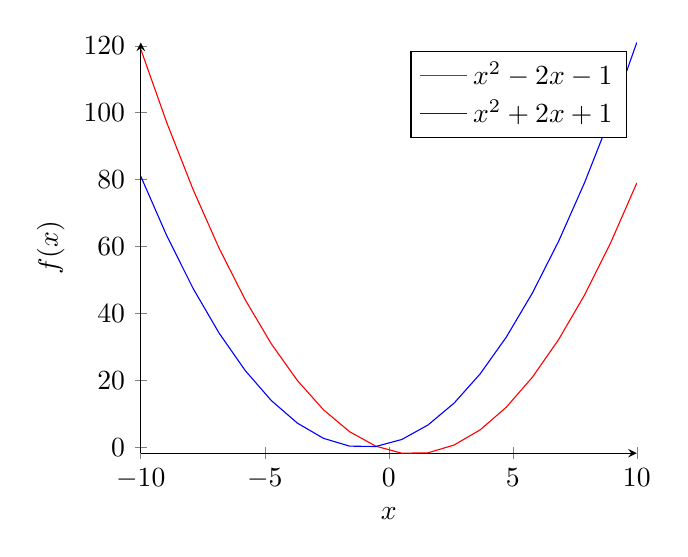
\begin{tikzpicture}
      \begin{axis}[
          width=0.65\textwidth,
          axis lines = left,
          xlabel = \(x\),
          ylabel = {\(f(x)\)},
      ]
        %Below the red parabola is defined
        \addplot [
            domain=-10:10, 
            samples=20, 
            color=red,
        ]
        {x^2 - 2*x - 1};
        \addlegendentry{\(x^2 - 2x - 1\)}
        %Here the blue parabola is defined
        \addplot [
            domain=-10:10, 
            samples=20, 
            color=blue,
            ]
            {x^2 + 2*x + 1};
        \addlegendentry{\(x^2 + 2x + 1\)}
      \end{axis}
    \end{tikzpicture}
    \caption{Plot of two parabola.}\label{fig:parabolaplot}
  \end{figure}
  
  \begin{figure}[htb!]
    \centering
    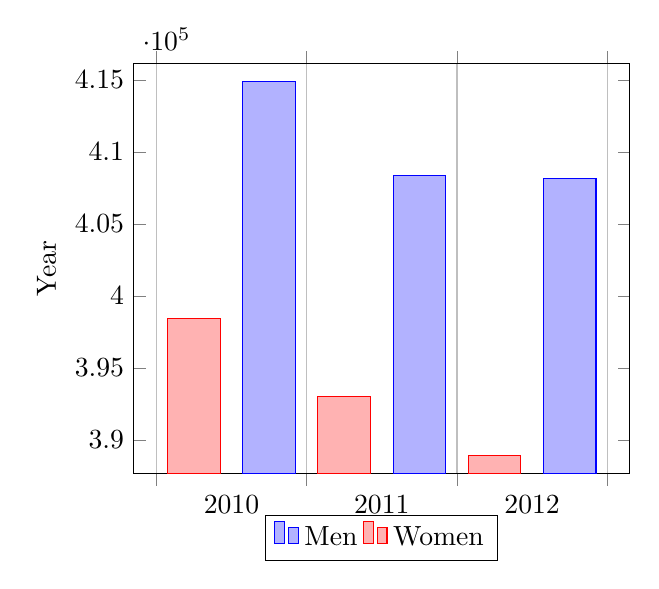
\begin{tikzpicture}
      \begin{axis}[
        width=0.65\textwidth,
        x tick label style={
          /pgf/number format/1000 sep=},
        ylabel=Year,
        enlargelimits=0.05,
        legend style={at={(0.5,-0.1)},
        anchor=north,legend columns=-1},
        ybar interval=0.7,
      ]
      \addplot 
        coordinates {(2012,408184) (2011,408348)
           (2010,414870) (2009,412156)};
      \addplot 
        coordinates {(2012,388950) (2011,393007) 
          (2010,398449) (2009,395972)};
      \legend{Men,Women}
      \end{axis}
    \end{tikzpicture}
    \caption{Example of a Bar Graph.}\label{fig:bargraph}
  \end{figure}
  
  \begin{figure}[htb!]
    \centering
    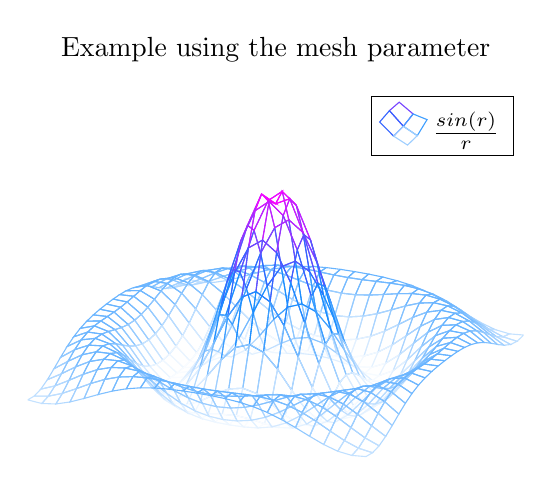
\begin{tikzpicture}
      \begin{axis}[
          width=0.65\textwidth,
          title=Example using the mesh parameter,
          hide axis,
          colormap/cool,
      ]
      \addplot3[
          mesh,
          samples=25,
          domain=-8:8,
      ]
      {sin(deg(sqrt(x^2+y^2)))/sqrt(x^2+y^2)};
      \addlegendentry{\(\frac{sin(r)}{r}\)}
      \end{axis}
    \end{tikzpicture}
    \caption{Example of a 3D Plot}\label{fig:3dplot}
  \end{figure}
  
  \begin{figure}[htb!]
    \centering
    \begin{tikzpicture}
      \begin{axis}[
          width=0.65\textwidth,
          enlargelimits=true,
      ]
      \addplot+[
          only marks,
          scatter,
          mark=*,
          mark size=2.9pt]
      table[meta=ma]
      {./Chapters/scattered_example.dat};
      \end{axis}
      \end{tikzpicture}
    \caption{Example of a Scatter Plot.}\label{fig:scatterplot}
  \end{figure}
  
  \clearpage
  \section{Equations}
  The following equation has no referencing number:
  \nonumeq{E & = m\ c^2}
  
  \Cref{eq:quickEq} has a reference to it though. Or for more control the source for \Cref{eq:quickEq} can be written out fully as it was for \Cref{eq:quickEq2}.
  
  \numeq{pi & = 3.1415...}{eq:quickEq} % shorthand for the following way of writing equations.
  \begin{align}\label{eq:quickEq2}
    e & = 2.7183...
  \end{align}
  
  If you have multiple equations that you want arranged very neatly, use the align environment and you can assign individual equations numbers as shown in \Cref{eq:multiref:a,eq:multiref:b,eq:multiref:c}.
  \begin{align}%Note: Alignment happens at the "=" character
    \label{eq:multiref:a} Equation1 & = 1\\
    \label{eq:multiref:b} Equation2 & = 2 + 2\\
    \label{eq:multiref:c} Equation3 & = 3 + 3 + 3
  \end{align}
  
  
  
  \printreferences % Add a Reference Section to the end of the Chapter.

\bigskip 
\clearpage\singlespacing

%%%%%%%%%%%%%%%%%%%%%%%%%%%%%%%%%%%%%%%%%%%%%%%%%%%%%%%%%%%%%%%%%%%%%%%%%%%%%%%%
%                                 BIBLIOGRAPHY                                 %
%%%%%%%%%%%%%%%%%%%%%%%%%%%%%%%%%%%%%%%%%%%%%%%%%%%%%%%%%%%%%%%%%%%%%%%%%%%%%%%%
%\nocite{*}  % Uncomment if you have a bibliography with work read but not cited
\printbibliography[heading=bibintoc]
\bigskip

%%%%%%%%%%%%%%%%%%%%%%%%%%%%%%%%%%%%%%%%%%%%%%%%%%%%%%%%%%%%%%%%%%%%%%%%%%%%%%%%
%                                  APPENDICES                                  %
%%%%%%%%%%%%%%%%%%%%%%%%%%%%%%%%%%%%%%%%%%%%%%%%%%%%%%%%%%%%%%%%%%%%%%%%%%%%%%%%
\appendix
\chapter{First Appendix}\label{app:}
  \section{Section 1}\label{sec:}
    \lipsum[34-36]
  \section{Section 2}\label{sec:}
    \lipsum[38]

\chapter{Second Appendix}\label{app:}
  \section{Section 1}\label{sec:}
    \lipsum[34-36]
  \section{Section 2}\label{sec:}
    \lipsum[38]

\insertappendix{Appendix_Name}

\insertappendix{PDF_Appendix}

\end{document}
